\documentclass[border=10pt]{standalone}
\usepackage[T1]{fontenc}
\usepackage{tikz}
\usepackage[svgnames]{xcolor}
\usetikzlibrary{arrows.meta, positioning, calc}

\colorlet{OrangeFill}{LightSalmon}
\colorlet{OrangeLine}{DarkSalmon!30!Chocolate}
\colorlet{GreenFill}{MediumAquamarine}
\colorlet{GreenLine}{MediumAquamarine!30!Teal}
\colorlet{PurpleFill}{MediumPurple}
\colorlet{PurpleLine}{MediumPurple!30!SlateBlue}
\colorlet{PinkFill}{Thistle}
\colorlet{PinkLine}{Thistle!30!Plum}
\colorlet{BlueFill}{LightSkyBlue}
\colorlet{BlueLine}{SteelBlue}
\colorlet{GrayFill}{LightGray!60!OldLace}
\colorlet{GrayLine}{RosyBrown!50!Silver}

\begin{document}
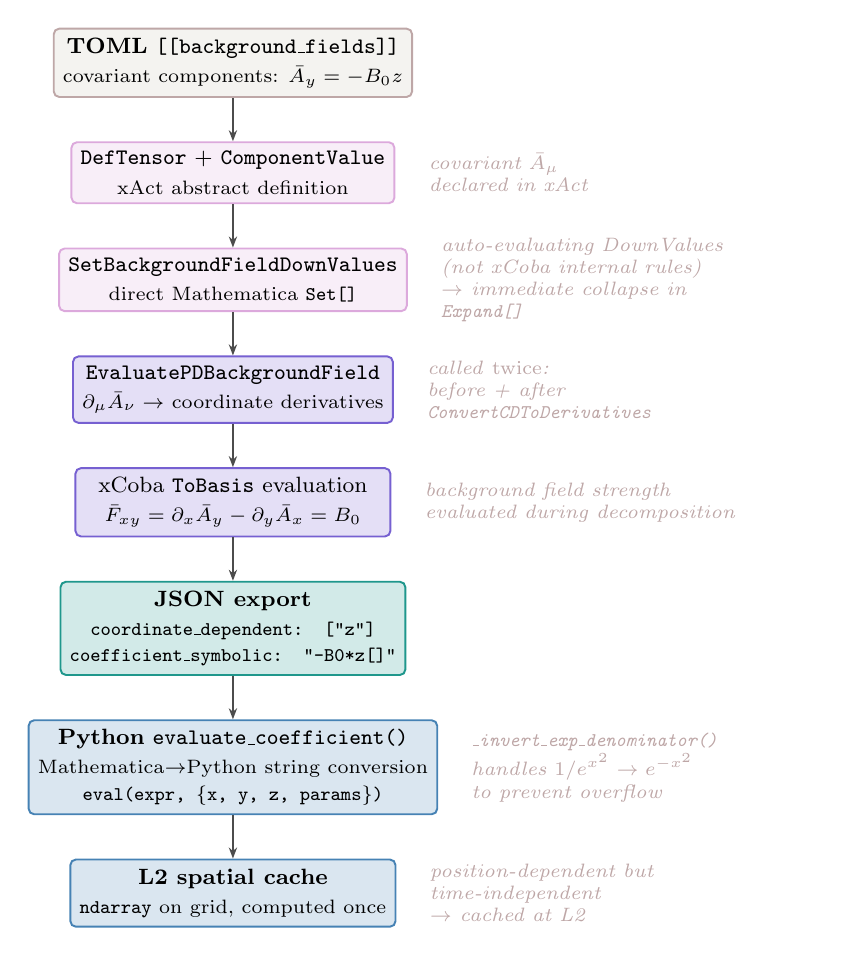
\begin{tikzpicture}[
    stage/.style={
        rectangle, rounded corners=2pt, minimum width=4.0cm,
        minimum height=0.7cm, draw=#1, line width=0.7pt,
        fill=#1!20, font=\footnotesize, align=center,
        text opacity=1, text=black
    },
    stage/.default={black!70},
    annot/.style={font=\scriptsize\itshape, text=GrayLine, align=left,
                  text width=4.4cm},
    arr/.style={-{Stealth[length=4pt, width=3pt]}, semithick, black!70},
    node distance=0.55cm
]

% Stages
\node[stage=GrayLine, fill=GrayFill, fill opacity=0.4] (toml)
    {\textbf{TOML} \texttt{[[background\_fields]]}\\[1pt]
     \scriptsize covariant components: $\bar{A}_y = -B_0 z$};

\node[stage=PinkLine, below=of toml] (wls)
    {\texttt{DefTensor} + \texttt{ComponentValue}\\[1pt]
     \scriptsize xAct abstract definition};
\node[annot, right=0.3cm of wls.east, anchor=west]
    {covariant $\bar{A}_\mu$\\declared in xAct};

\node[stage=PinkLine, below=of wls] (downval)
    {\texttt{SetBackgroundFieldDownValues}\\[1pt]
     \scriptsize direct Mathematica \texttt{Set[]}};
\node[annot, right=0.3cm of downval.east, anchor=west]
    {auto-evaluating DownValues\\(not xCoba internal rules)\\$\to$ immediate collapse in\\
     \texttt{Expand[]}};

\node[stage=PurpleLine, below=of downval] (evalPD)
    {\texttt{EvaluatePDBackgroundField}\\[1pt]
     \scriptsize $\partial_\mu \bar{A}_\nu \to$ coordinate derivatives};
\node[annot, right=0.3cm of evalPD.east, anchor=west]
    {called \emph{twice}:\\before + after\\
     \texttt{ConvertCDToDerivatives}};

\node[stage=PurpleLine, below=of evalPD] (tobasis)
    {xCoba \texttt{ToBasis} evaluation\\[1pt]
     \scriptsize $\bar{F}_{xy} = \partial_x \bar{A}_y - \partial_y \bar{A}_x = B_0$};
\node[annot, right=0.3cm of tobasis.east, anchor=west]
    {background field strength\\evaluated during decomposition};

\node[stage=GreenLine, below=of tobasis] (json)
    {\textbf{JSON export}\\[1pt]
     \scriptsize \texttt{coordinate\_dependent: ["z"]}\\
     \scriptsize \texttt{coefficient\_symbolic: "-B0*z[]"}};

\node[stage=BlueLine, below=of json] (pyeval)
    {\textbf{Python} \texttt{evaluate\_coefficient()}\\[1pt]
     \scriptsize Mathematica$\to$Python string conversion\\
     \scriptsize \texttt{eval(expr, \{x, y, z, params\})}};
\node[annot, right=0.3cm of pyeval.east, anchor=west]
    {\texttt{\_invert\_exp\_denominator()}\\
     handles $1/e^{x^2} \to e^{-x^2}$\\to prevent overflow};

\node[stage=BlueLine, below=of pyeval] (cache)
    {\textbf{L2 spatial cache}\\[1pt]
     \scriptsize \texttt{ndarray} on grid, computed once};
\node[annot, right=0.3cm of cache.east, anchor=west]
    {position-dependent but\\time-independent\\$\to$ cached at L2};

% Arrows
\foreach \a/\b in {toml/wls, wls/downval, downval/evalPD,
                   evalPD/tobasis, tobasis/json, json/pyeval, pyeval/cache} {
    \draw[arr] (\a) -- (\b);
}

\end{tikzpicture}
\end{document}
